\section{Schematic Implementation}
Following the architectural analysis discussed in the previous chapter, this section details the transistor-level implementation of the 32~GBaud Voltage-Mode Source-Series Terminated (SST) transmitter. 

\subsection{Unit Slice Architecture}
The fundamental building block of the entire driver array is this unit slice. As illustrated in Figure~\ref{fig:unit_slice}, the slice is composed of an inverter and series resistance.

\begin{figure}[H]
    \centering
    
\includegraphics[width=0.99\textwidth]{Single Slice schematic.png}
    \caption{Schematic of the Single-Ended (SE) unit slice.}
    \label{fig:unit_slice}
\end{figure}

A critical design parameter within this unit slice is the internal impedance distribution. 
To meet PCIe Gen 6.0 specifications, the transmitter provides a nominal $50~\Omega$ single-ended termination. 
This $50~\Omega$ target is partitioned such that the ratio between the series poly resistor ($R_{series}$) and 
the transistor ON-resistance ($R_{on}$) is approximately 80\% and 20\%, respectively. 

By forcing the passive resistor (${\sim}40~\Omega$) to dominate the total output impedance, 
the variations of the transistor's $R_{on}$ (${\sim}10~\Omega$) across different output voltage swings are attenuated. 
This 80/20 ratio is sized and preserved across all manufacturing process corners, 
forming the baseline for the driver's Signal-to-Distortion Ratio (SDR). and Ratio level mismatch (RLM)

To ensure the transmitter maintains the required impedance characteristics across all manufacturing process corners, 
a digital calibration scheme is employed. The design utilizes transmission gates (TGs) as switches to manage the impedance network, 
to maintain VGS=VDD whatever the i/p

\subsection{Calibration Architecture}
As shown in Figure~\ref{fig:calibration_schematic}, the driver employs a parallel branch architecture to provide 
an additional degree of freedom for the input pair. The design philosophy centers on ensuring that the series resistance ($R_{series}$) 
is intentionally sized to be larger than the target resistance ($R_{desired}$). This approach ensures that at the Fast-Fast (FF) process corner, 
the effective impedance remains close to $R_{desired}$ without requiring the opening of calibration banks. 

By guaranteeing specific sizing for the polysilicon resistors ($R_{poly}$), we achieve uniform incremental steps across process variations. 
Specifically, at the Typical-Typical (TT) corner, a single calibration step is sufficient to achieve $R_{desired}$, 
whereas at the Slow-Slow (SS) corner, two branches of the calibration DAC are activated to compensate for the higher resistance.

\begin{figure}[H]
    \centering
    
\includegraphics[width=1.1\textwidth]{Callibrated slice.png}
    \caption{Schematic representation of the digitally calibrated driver slice.}
    \label{fig:calibration_schematic}
\end{figure}

\newpage

The resistance variations observed across different process corners are illustrated in Figure~\ref{fig:R2_variation}. This data serves as the baseline for the subsequent calibration design.

\begin{figure}[H]
    \centering
    
\includegraphics[width=0.9\textwidth]{R_value_changing.png}
    \caption{Resistance variation across process corners for output R2.}
    \label{fig:R2_variation}
\end{figure}

The calibration logic is designed to maintain the 80/20 impedance partitioning ratio. For a nominal impedance of $396.875~\Omega$ (derived from the $50~\Omega$ system requirement), $R_{series}$ is targeted at approximately $320~\Omega$. 

To ensure consistent performance, the base series resistor is selected as $470~\Omega$. This selection yields a nominal $320~\Omega$ at the FF corner and $620~\Omega$ at the SS corner, providing an equal step size of $150~\Omega$ across the operating range. The bank resistance ($R_{bank}$) calculation follows the parallel combination rule:

\begin{equation}
    R_{TT} = \frac{R_{series} \cdot R_{bank}}{R_{series} + R_{bank}} \approx 320~\Omega
\end{equation}

Solving for $R_{bank}$ yields a required value of approximately $1003~\Omega$. To maintain consistent variation percentages between $R_{bank}$ and $R_{series}$, $R_{bank}$ is implemented using the same unit resistance sizing as $R_{series}$, configured with two series $R_{poly}$ elements and a $60~\Omega$ TG resistance contribution. 

Verification of this logic for the SS corner is confirmed by:

\begin{equation}
    R_{SS} = \frac{620 \cdot \left( \frac{1003}{2} \right) \cdot \left( \frac{620}{470} \right)}{620 + \left( \frac{1003}{2} \right) \cdot \left( \frac{620}{470} \right)} \approx 320~\Omega
\end{equation}

\newpage
\subsection{Parasitics Reduction Techniques}
\label{sec:parasitics_reduction}

To optimize the high-speed performance of the transmitter, a strategic approach to parasitic reduction was implemented within the impedance calibration network. Conventional designs often utilize identical parallel slices, which leads to excessive parasitic capacitance, particularly in the high-resistance calibration banks.

As illustrated in Figure~\ref{fig:parasitics_comparison}, the implemented design utilizes a segmented DAC topology. Rather than maintaining uniform slice scaling for the polysilicon resistors ($R_{poly}$), the DAC is divided into series resistance elements for the Least Significant Bits (LSBs) and parallel resistance elements for the Most Significant Bits (MSBs). 

\begin{figure}[H]
    \centering
    \begin{subfigure}[b]{0.5\textwidth}
        \centering
        
\includegraphics[width=\textwidth]{schematic1.png}
        \caption{Initial DAC schematic.}
    \end{subfigure}
    \hfill
    \begin{subfigure}[b]{0.45\textwidth}
        \centering
        
\includegraphics[width=\textwidth]{schematic2.png}
        \caption{modified DAC schematic.}
    \end{subfigure}
    
    \vspace{0.5cm}
    
    \begin{subfigure}[b]{0.5\textwidth}
        \centering
        
\includegraphics[width=\textwidth]{eye1.png}
        \caption{Eye diagram with high parasitic loading.}
    \end{subfigure}
    \hfill
    \begin{subfigure}[b]{0.45\textwidth}
        \centering
        
\includegraphics[width=\textwidth]{eye2.png}
        \caption{Eye diagram with optimized parasitic loading.}
    \end{subfigure}
    \caption{Parasitic reduction strategy using a segmented DAC architecture and the resulting impact on eye diagram quality.}
    \label{fig:parasitics_comparison}
\end{figure}

The rationale for this architectural decision is twofold:
\begin{enumerate}
    \item \textbf{Parasitic Minimization:} While this configuration results in a slight increase in parasitics for the LSBs, the total parasitic capacitance of the entire bank is significantly reduced, which is essential for maintaining the bandwidth required for PCIe Gen 6.0 data rates.
    \item \textbf{Segmentation Logic:} The DAC segmentation occurs starting from the $B_4$ bit rather than the middle ($B_3$). This prioritization acknowledges that MSBs dominate the impedance calibration process; because $R_{bank}$ is substantially higher than $R_{main}$, the MSBs contribute more significantly to the overall output impedance variation. Consequently, minimizing parasitics for the MSBs is prioritized.
\end{enumerate}

Additionally, a common $R_{poly}$ unit is employed for both N-type and P-type segments to ensure process matching and simplify the layout geometry. This design optimization is verified by the improved eye diagram opening shown in Figure~\ref{fig:parasitics_comparison}, which demonstrates the reduction in signal distortion achieved through lower overall capacitive loading.
\newline


Table~\ref{tab:dac_segmentation} quantifies the number of resistive elements ($R$) assigned to the main branch ($M$) and the calibration branches ($B_0, B_1$) for different segmentation strategies. The total resistive count provided at the bottom of each column reflects the design complexity and corresponding parasitic footprint for each case.

\begin{table}[H]
    \centering
    \renewcommand{\arraystretch}{1.2}
    \begin{tabular}{l c c c c c c c c c}
        \toprule
        & \multicolumn{3}{c}{\textbf{Divide from $B_3$}} & \multicolumn{3}{c}{\textbf{Divide from $B_4$}} & \multicolumn{3}{c}{\textbf{Divide from $B_5$}} \\
        \cmidrule(lr){2-4} \cmidrule(lr){5-7} \cmidrule(lr){8-10}
        Weight & $M$ & $B_0$ & $B_1$ & $M$ & $B_0$ & $B_1$ & $M$ & $B_0$ & $B_1$ \\
        \midrule
        64 & 8 & 16 & 16 & 4 & 8 & 8 & 2 & 4 & 4 \\
        32 & 4 & 8 & 8 & 2 & 4 & 4 & 1 & 2 & 2 \\
        16 & 2 & 4 & 4 & 1 & 2 & 2 & 2 & 4 & 4 \\
        8 & 1 & 2 & 2 & 2 & 4 & 4 & 4 & 8 & 8 \\
        4 & 2 & 4 & 4 & 4 & 8 & 8 & 8 & 16 & 16 \\
        2 & 4 & - & - & 8 & - & - & 16 & - & - \\
        1 & 8 & - & - & 16 & - & - & 32 & - & - \\
        \midrule
        \textbf{Total} & \textbf{29} & \textbf{34} & \textbf{34} & \textbf{37} & \textbf{26} & \textbf{26} & \textbf{65} & \textbf{34} & \textbf{34} \\
        \textbf{Sum} & \multicolumn{3}{c}{\textbf{97}} & \multicolumn{3}{c}{\textbf{89}} & \multicolumn{3}{c}{\textbf{133}} \\
        \bottomrule
    \end{tabular}
    \caption{Distribution of resistive elements across DAC branches for various segmentation points.}
    \label{tab:dac_segmentation}
\end{table}

As the data illustrates, segmenting the DAC from $B_4$ provides the optimal configuration with a total count of 89 resistive elements, achieving the lowest overall parasitic contribution compared to the $B_3$ and $B_5$ approaches. This configuration effectively balances the design complexity with the necessity of maintaining low-parasitic paths for the MSBs.
\newpage
\subsection{Monotonicity Verification}
\label{sec:monotonicity}

To ensure the linearity and monotonic behavior of the DAC across process and mismatch variations, a series of Monte-Carlo simulations were conducted. The monotonicity check involves applying a ramp input signal to the DAC and monitoring the Differential Non-Linearity (DNL) to ensure it remains within specified bounds.

\begin{figure}[H]
    \centering
    \begin{subfigure}[b]{0.6\textwidth}
        \centering
        
\includegraphics[width=\textwidth]{DNL_ideal.jpg}
        \caption{DNL characteristic curve across the output range. without montecarlo}
    \end{subfigure}
    \hfill
    \begin{subfigure}[b]{0.35\textwidth}
        \centering
        
\includegraphics[width=\textwidth]{DNL_max_min.png}
        \caption{DNL limits comparison with binary then 2b to 3 th}
    \end{subfigure}
    \caption{Monotonicity verification using Monte-Carlo analysis for binary and segmented DAC configurations.}
    \label{fig:monotonicity_check}
\end{figure}

As shown in Figure~\ref{fig:monotonicity_check}, the segmented DAC architecture, utilizing a conversion from 2 binary bits to 3 thermometer bits ($2b \rightarrow 3T$), provides a significant improvement in linearity. The performance summary is as follows:

\begin{itemize}
    \item \textbf{Binary DAC:} The observed DNL range was $[-1.158, 1.084]~\text{LSB}$, indicating potential non-monotonicity due to the DNL exceeding $1~\text{LSB}$.
    \item \textbf{Segmented DAC ($2b \rightarrow 3T$):} The DNL range is effectively reduced to $[-0.961, 0.975]~\text{LSB}$. 
\end{itemize}

By maintaining the DNL within $\pm 1~\text{LSB}$, the segmented DAC architecture guarantees monotonicity. This improvement confirms the efficacy of the $2b \rightarrow 3T$ segmentation in mitigating the impact of component mismatch on the overall DAC transfer function.


\newpage
\subsection*{DAC Bit Configuration and Testbench Architecture}
\label{sec:dac_tb}


\begin{figure}[H]
    \centering
    \begin{subfigure}[b]{0.9\textwidth}
        \centering
        
\includegraphics[width=\textwidth]{DAC Bits.png}
        \caption{Unit DAC bit slice configurations.}
        \label{fig:dac_bits}
    \end{subfigure}
    
    \vspace{0.5cm}
    
    \begin{subfigure}[b]{0.9\textwidth}
        \centering
        
\includegraphics[width=\textwidth]{TB.png}
        \caption{General testbench environment for DAC characterization.}
        \label{fig:tb_overview}
    \end{subfigure}
    \caption{DAC bit architecture and corresponding testbench setup.}
    \label{fig:dac_and_tb}
\end{figure}

\begin{itemize}
    \item \textbf{Stimulus Generation:} The input block is highly configurable, enabling the generation of NRZ, PAM4, and DC signals to perform transient, AC, and linearity measurements as required by the design specifications.
    \item \textbf{Calibration Control:} The calibration code block provides the necessary digital control signals to the calibration banks, allowing for post-layout verification of the impedance tuning range.
    \item \textbf{Power Delivery:} The design operates on a nominal supply voltage ($V_{DD}$) of $0.9~\text{V}$, sourced from an integrated regulator to maintain the required output voltage swing across all process, voltage, and temperature (PVT) corners.
    \item \textbf{Load Modeling:} To accurately emulate the channel environment, the output stage is loaded with an equivalent model representing the system-level interface, characterized by $150~\text{fF}$ (ESD protection), 70f after driver and 80f after inductor , $50~\text{fF}$ (pad capacitance), $300~\text{pH}$ (package inductance), $250~\text{m}\Omega$ (package resistance), and $75~\text{fF}$ (package capacitance).
\end{itemize}

\subsection{Inductor Design and Modeling}
\label{sec:inductor_design}

\begin{figure}[H]
    \centering
    \begin{subfigure}[b]{0.45\textwidth}
        \centering
        
\includegraphics[width=\textwidth]{Inductor test bench.png}
        \caption{Inductor behavioral model schematic.}
    \end{subfigure}
    \hfill
    \begin{subfigure}[b]{0.45\textwidth}
        \centering
        
\includegraphics[width=\textwidth]{LRC eqns.png}
        \caption{Variable modeling parameters ($L_{des}, C_{bb}, R_{bb}$).}
    \end{subfigure}
    
    \vspace{0.5cm}
    
    \begin{subfigure}[b]{0.42\textwidth}
        \centering
        
\includegraphics[width=\textwidth]{Differential Impedance.png}
        \caption{Differential impedance vs. $L_{des}$.}
    \end{subfigure}
    \hfill
    \begin{subfigure}[b]{0.45\textwidth}
        \centering
        
\includegraphics[width=\textwidth]{Differential RL.png}
        \caption{Differential return loss vs. $L_{des}$.}
    \end{subfigure}
    \caption{Peaking inductor design and optimization using behavioral modeling.}
    \label{fig:inductor_design}
\end{figure}

The modeling approach captures the physical characteristics of the inductor by extracting the Peak Quality Factor (PQF) and Self-Resonant Frequency (SRF) from EMX  of premade inductor. to allow efficient iterative design . These values are translated into parasitic components ($R$ and $C$) using the following design equations:

\begin{equation}
    \text{PQF} = \frac{\omega L}{R}
\end{equation}

\begin{equation}
    R = \frac{\omega \cdot \text{PQF} \cdot L}{\text{PQF}} \quad \text{and} \quad C = \frac{1}{\omega_{\text{SRF}}^2 \cdot L}
\end{equation}

To optimize performance, $L_{des}$ was swept, as shown in Figures~\ref{fig:inductor_design}(b) and (c), to identify the value that achieves the optimal RL accross corners

\newpage
\subsection{Final Inductor Implementation and Verification}
\label{sec:inductor_final}

\begin{figure}[H]
    \centering
    % Top row: Layout
    \begin{subfigure}[b]{0.6\textwidth}
        \centering
        
\includegraphics[width=\textwidth]{Inductor Layout.png}
        \caption{Physical inductor layout.}
    \end{subfigure}
    
    \vspace{0.5cm}
    
    % Bottom row: Graphs
    \begin{subfigure}[b]{0.45\textwidth}
        \centering
        
\includegraphics[width=\textwidth]{Lsim.png}
        \caption{Simulated inductance ($L_{sim}$) vs. frequency.}
    \end{subfigure}
    \hfill
    \begin{subfigure}[b]{0.45\textwidth}
        \centering
        
\includegraphics[width=\textwidth]{Qsim.png}
        \caption{Simulated quality factor ($Q_{sim}$) vs. frequency.}
    \end{subfigure}
    \caption{Finalized peaking inductor layout and electromagnetic simulation results.}
    \label{fig:inductor_final}
\end{figure}

The physical design, shown in Figure~\ref{fig:inductor_final}(a), was validated using EMX to confirm that the inductance and quality factor ($Q$) meet the design requirements. As illustrated in Figures~\ref{fig:inductor_final}(b) and (c), the simulation results demonstrate stable inductive behavior and a high-Q profile, ensuring that the peaking network effectively enhances the transmitter bandwidth without introducing excessive loss or impedance mismatch at the Nyquist operating point.

\section{Pre layout Simulation}
\subsection{Output Voltage Swing (NRZ) Corner Analysis}
\label{sec:swing_results}

The output voltage swing was characterized across various process corners to ensure compliance with the target specification of $0.8~\text{V}$ to $1.0~\text{V}$ (differential). Figure~\ref{fig:nrz_swing_corners} illustrates the performance distribution across the Typical-Typical (TT), fast-slow corners, and extreme corner variations.

\begin{figure}[H]
    \centering
    % Row 1: TT Corner
    \begin{subfigure}[b]{0.65\textwidth}
        
\includegraphics[width=\textwidth]{TT_Swing.png}
    \end{subfigure}
    \begin{subfigure}[b]{0.30\textwidth}
        
\includegraphics[width=\textwidth]{magnified_TT_Swing.png}
    \end{subfigure}
    \caption*{Swing performance at the TT corner.}
    
    \vspace{0.3cm}
    
    % Row 2: SS/FF Corners
    \begin{subfigure}[b]{0.65\textwidth}
        
\includegraphics[width=\textwidth]{FF_SS_Swing.png}
    \end{subfigure}
    \begin{subfigure}[b]{0.30\textwidth}
        
\includegraphics[width=\textwidth]{magnified_FF_SS_Swing.png}
    \end{subfigure}
    \caption*{Swing performance at SS and FF corners.}
    
    \vspace{0.3cm}
    
    % Row 3: SF/FS Corners
    \begin{subfigure}[b]{0.65\textwidth}
        
\includegraphics[width=\textwidth]{SF_FS_Swing.png}
    \end{subfigure}
    \begin{subfigure}[b]{0.30\textwidth}
        
\includegraphics[width=\textwidth]{magnified_SF_FS_Swing.png}
    \end{subfigure}
    \caption*{Swing performance at SF and FS corners.}
    
    \caption{NRZ output voltage swing analysis across process corners.}
    \label{fig:nrz_swing_corners}
\end{figure}

The simulation results confirm that the transmitter maintains a consistent swing within the required range across all process variations, validating the calibration strategy's effectiveness in compensating for device mismatch.


\subsection{PAM4 Eye Diagrams}
Some of the simulated differential eye diagrams across the process corners are presented in Figure~\ref{fig:pam4_corners}.

\begin{figure}[H]
    \centering
    \begin{subfigure}[b]{0.48\textwidth}
        \centering
        
\includegraphics[width=\textwidth]{PAM4_Nominal_EYE.png}
        \caption{Nominal (TT) Corner}
        \label{fig:pam4_tt}
    \end{subfigure}
    \hfill
    \begin{subfigure}[b]{0.48\textwidth}
        \centering
        
\includegraphics[width=\textwidth]{PAM4_FFmin_EYE.png}
        \caption{FFmin Corner}
        \label{fig:pam4_ff}
    \end{subfigure}
    
    \vspace{0.5cm}
    
    \begin{subfigure}[b]{0.48\textwidth}
        \centering
        
\includegraphics[width=\textwidth]{PAM4_SSmax_EYE.png}
        \caption{SSmax Corner}
        \label{fig:pam4_ss}
    \end{subfigure}
    \hfill
    \begin{subfigure}[b]{0.48\textwidth}
        \centering
        
\includegraphics[width=\textwidth]{PAM4_SFmin_EYE.png}
        \caption{SFmin Corner}
        \label{fig:pam4_sf}
    \end{subfigure}
    
    \vspace{0.5cm}
    
    \begin{subfigure}[b]{0.48\textwidth}
        \centering
        
\includegraphics[width=\textwidth]{PAM4_FSmax_EYE.png}
        \caption{FSmax Corner}
        \label{fig:pam4_fs}
    \end{subfigure}
    
    \caption{32~GBaud PAM4 differential eye diagrams across standard process corners.}
    \label{fig:pam4_corners}
\end{figure}

\subsection{Level Separation Mismatch Ratio ($R_{LM}$)}
Transmitter linearity is quantified using the Level Separation Mismatch Ratio ($R_{LM}$). It evaluates the uniformity of the three eye openings ($\Delta V_{top}, \Delta V_{mid}, \Delta V_{bot}$) relative to the total peak-to-peak voltage swing ($V_{swing}$). The formula is defined as:

\begin{equation}
    R_{LM} = \frac{3 \cdot \min(\Delta V_{top}, \Delta V_{mid}, \Delta V_{bot})}{V_{swing}}
\end{equation}

The extracted voltage levels and the calculated $R_{LM}$ for each process corner are summarized in Table~\ref{tab:rlm_summary}.

\begin{table}[H]
    \centering
    \caption{Summary of PAM4 Linearity ($R_{LM}$) Across Process Corners}
    \label{tab:rlm_summary}
    \renewcommand{\arraystretch}{1.3} % Adds vertical spacing
    \begin{tabular}{lccc}
        \toprule
        \textbf{Process Corner} & \textbf{Peak-to-Peak Swing ($V_{swing}$)} & \textbf{Minimum Eye Opening} & \textbf{$R_{LM}$} \\
        \midrule
        \textbf{Nominal (TT)} & $902.51~\mV$ & $297.33~\mV$ & \textbf{0.988} \\
        \textbf{FFmin}        & $995.10~\mV$ & $330.13~\mV$ & \textbf{0.995} \\
        \textbf{SSmax}        & $808.36~\mV$ & $261.95~\mV$ & \textbf{0.972} \\
        \textbf{SFmin}        & $994.91~\mV$ & $326.45~\mV$ & \textbf{0.984} \\
        \textbf{FSmax}        & $807.44~\mV$ & $265.14~\mV$ & \textbf{0.985} \\
        \bottomrule
    \end{tabular}
\end{table}

\subsection{Comprehensive Power Consumption across 45 PVT Corners}
To rigorously evaluate the power efficiency and stability of the transmitter, the total power consumption was extracted across all 45 Process, Voltage, and Temperature (PVT) corners. The analysis compares the driver's power dissipation when operating with a standard NRZ input versus the fully segmented 32~GBaud PAM4 input. 

Table~\ref{tab:power_tt_ss_ff} details the Typical-Typical (TT), Slow-Slow (SS), and Fast-Fast (FF) corners, while Table~\ref{tab:power_sf_fs} details the cross-corners, Slow-Fast (SF) and Fast-Slow (FS).

\begin{table}[H]
    \centering
    \small
    \caption{Power Consumption (NRZ vs. PAM4) - TT, SS, and FF Corners}
    \label{tab:power_tt_ss_ff}
    \renewcommand{\arraystretch}{1.1}
    \begin{tabular}{llcc}
        \toprule
        \textbf{Process} & \textbf{Corner Variation} & \textbf{NRZ Power (mW)} & \textbf{PAM4 Power (mW)} \\
        \midrule
        \textbf{TT} & nom & 8.288 & 10.220 \\
                    & max & 6.817 & 8.364 \\
                    & VDDp\_T0 & 9.953 & 12.290 \\
                    & VDDp\_Tp & 10.050 & 12.360 \\
                    & VDD0\_Tn & 8.291 & 10.240 \\
                    & VDD0\_Tp & 8.354 & 10.270 \\
                    & VDDn\_Tn & 6.789 & 8.366 \\
                    & VDDn\_T0 & 6.776 & 8.336 \\
                    & min & 9.944 & 12.300 \\
        \midrule
        \textbf{SS} & nom & 8.750 & 10.770 \\
                    & max & 7.136 & 8.742 \\
                    & VDDp\_T0 & 10.520 & 12.970 \\
                    & VDDp\_Tp & 10.550 & 12.990 \\
                    & VDD0\_Tn & 8.774 & 10.810 \\
                    & VDD0\_Tp & 8.765 & 10.770 \\
                    & VDDn\_Tn & 7.155 & 8.779 \\
                    & VDDn\_T0 & 7.130 & 8.748 \\
                    & min & 10.530 & 13.000 \\
        \midrule
        \textbf{FF} & nom & 7.933 & 9.794 \\
                    & max & 6.584 & 8.071 \\
                    & VDDp\_T0 & 9.531 & 11.770 \\
                    & VDDp\_Tp & 9.693 & 11.900 \\
                    & VDD0\_Tn & 7.909 & 9.793 \\
                    & VDD0\_Tp & 8.062 & 9.894 \\
                    & VDDn\_Tn & 6.470 & 8.001 \\
                    & VDDn\_T0 & 6.486 & 7.993 \\
                    & min & 9.505 & 11.770 \\
        \bottomrule
    \end{tabular}
\end{table}

\begin{table}[H]
    \centering
    \small
    \caption{Power Consumption (NRZ vs. PAM4) - SF and FS Corners}
    \label{tab:power_sf_fs}
    \renewcommand{\arraystretch}{1.1}
    \begin{tabular}{llcc}
        \toprule
        \textbf{Process} & \textbf{Corner Variation} & \textbf{NRZ Power (mW)} & \textbf{PAM4 Power (mW)} \\
        \midrule
        \textbf{SF} & nom & 8.286 & 10.220 \\
                    & max & 6.817 & 8.366 \\
                    & VDDp\_T0 & 9.948 & 12.290 \\
                    & VDDp\_Tp & 10.050 & 12.360 \\
                    & VDD0\_Tn & 8.291 & 10.250 \\
                    & VDD0\_Tp & 8.352 & 10.270 \\
                    & VDDn\_Tn & 6.792 & 8.369 \\
                    & VDDn\_T0 & 6.777 & 8.340 \\
                    & min & 9.941 & 12.300 \\
        \midrule
        \textbf{FS} & nom & 8.279 & 10.210 \\
                    & max & 6.808 & 8.351 \\
                    & VDDp\_T0 & 9.949 & 12.280 \\
                    & VDDp\_Tp & 10.050 & 12.350 \\
                    & VDD0\_Tn & 8.281 & 10.230 \\
                    & VDD0\_Tp & 8.348 & 10.260 \\
                    & VDDn\_Tn & 6.775 & 8.341 \\
                    & VDDn\_T0 & 6.764 & 8.323 \\
                    & min & 9.938 & 12.290 \\
        \bottomrule
    \end{tabular}
\end{table}

\newpage
\subsection{Output Impedance and Return Loss Verification}
To ensure signal integrity and compliance with the PCIe Gen 6.0 standard, the transmitter's output impedance and return loss were extracted across all 45 Process, Voltage, and Temperature (PVT) corners. 

Figure~\ref{fig:rdiff} illustrates the differential output impedance ($R_{diff}$) versus frequency. The driver maintains a stable impedance profile tightly centered around the 100~$\Omega$ differential target across the required frequency band and all PVT variations.

\begin{figure}[H]
    \centering
    
\includegraphics[width=1.1\textwidth]{Rdiff.png}
    \caption{Differential output impedance ($R_{diff}$) across 45 PVT corners.}
    \label{fig:rdiff}
\end{figure}

Furthermore, the differential return loss ($S_{dd11}$) and common-mode return loss ($S_{cc11}$) must strictly adhere to the PCIe Gen 6.0 specified masks. Figure~\ref{fig:diff_rl} compares the simulated differential return loss against the standard mask, while Figure~\ref{fig:cm_rl} presents the common-mode return loss against its respective mask. The simulated results demonstrate that the transmitter maintains significant margin and successfully meets the stringent return loss specifications across all 45 corners up to the Nyquist frequency.

\begin{figure}[H]
    \centering
    \begin{subfigure}[b]{1\textwidth}
        \centering
        
\includegraphics[width=\textwidth]{Sdiff.png}
        \caption{Simulated $S_{dd11}$ across 45 corners}
        \label{fig:sdiff_sim}
    \end{subfigure}
    \hfill
    \begin{subfigure}[b]{1\textwidth}
        \centering
        
\includegraphics[width=\textwidth]{Diff_RL_Mask.png}
        \caption{PCIe Gen 6.0 Differential RL Mask}
        \label{fig:sdiff_mask}
    \end{subfigure}
    \caption{Differential Return Loss ($S_{dd11}$) verification.}
    \label{fig:diff_rl}
\end{figure}

\begin{figure}[H]
    \centering
    \begin{subfigure}[b]{1\textwidth}
        \centering
        
\includegraphics[width=\textwidth]{S11CM.png}
        \caption{Simulated $S_{cc11}$ across 45 corners}
        \label{fig:s11cm_sim}
    \end{subfigure}
    \hfill
    \begin{subfigure}[b]{1\textwidth}
        \centering
        
\includegraphics[width=\textwidth]{CM_RL.png}
        \caption{PCIe Gen 6.0 Common Mode RL Mask}
        \label{fig:s11cm_mask}
    \end{subfigure}
    \caption{Common Mode Return Loss ($S_{cc11}$) verification.}
    \label{fig:cm_rl}
\end{figure}

\newpage
\subsection{Single bit Response (SBR) Analysis}
To characterize the transmitter's impulse response and analyze the Total Harmonic Distortion (THD), 
a single pulse was applied to the differential inputs, $V_{inP}$ and $V_{inN}$. This characterization provides 
the essential data to determine the cursor ratios relative to the main cursor.

\begin{figure}[H]
    \centering
    \begin{subfigure}[b]{0.48\textwidth}
        \centering
        
\includegraphics[width=\textwidth]{VinP_SBR.png} % Ensure this is your VinP file
        \caption{Single bit input signal $V_{inP}$}
        \label{fig:vinp}
    \end{subfigure}
    \hfill
    \begin{subfigure}[b]{0.48\textwidth}
        \centering
        
\includegraphics[width=\textwidth]{VinN_SBR.png} % Ensure this is your VinN file
        \caption{Single bit input signal $V_{inN}$}
        \label{fig:vinn}
    \end{subfigure}
    \vspace{0.5cm}
    \begin{subfigure}[b]{0.95\textwidth}
        \centering
        
\includegraphics[width=\textwidth]{SBR.png}
        \caption{Single bit Response (SBR) graph}
        \label{fig:sbr_graph}
    \end{subfigure}
    \caption{Single Pulse Response characterization of the driver.}
    \label{fig:spr_analysis}
\end{figure}

The cursor values, normalized after DC shift ($+440.465\text{ mV}$), are summarized in Table~\ref{tab:spr_cursors}. 
Based on this analysis, the worst-case cursor configuration is identified as $00000000001\textcolor{red}{1}00$.

\begin{table}[H]
    \centering
    \caption{Cursor analysis and ratios after DC shift}
    \label{tab:spr_cursors}
    \renewcommand{\arraystretch}{1.2}
    \small
    \begin{tabular}{lccc}
        \toprule
        \textbf{Cursor Name} & \textbf{Raw Value (mV)} & \textbf{Value After DC Shift (mV)} & \textbf{Ratio} \\
        \midrule
        Pre-cursor h-2 (V13) & -440.465 & 0.000 & 0.0000 \\
        Pre-cursor h-1 (V12) & -440.471 & -0.006 & -0.0000 \\
        Main Cursor h0 (V1)  & 484.428  & 924.893 & 1.0000 \\
        Post-cursor h+1 (V2) & -490.964 & -50.499 & -0.0546 \\
        Post-cursor h+2 (V3) & -438.877 & 1.588 & 0.0017 \\
        Post-cursor h+3 (V4) & -437.229 & 3.236 & 0.0035 \\
        Post-cursor h+4 (V5) & -439.352 & 1.113 & 0.0012 \\
        Post-cursor h+5 (V6) & -440.107 & 0.358 & 0.0004 \\
        Post-cursor h+6 (V7) & -440.335 & 0.130 & 0.0001 \\
        Post-cursor h+7 (V8) & -440.411 & 0.054 & 0.0001 \\
        Post-cursor h+8 (V9) & -440.439 & 0.026 & 0.0000 \\
        Post-cursor h+9 (V10)& -440.449 & 0.016 & 0.0000 \\
        Post-cursor h+10 (V11)& -440.454 & 0.011 & 0.0000 \\
        \bottomrule
    \end{tabular}
\end{table}
\subsection{Signal-to-ISI Ratio (SIR) Analysis}
The transmitter's immunity to Inter-Symbol Interference (ISI) is quantified by the Signal-to-ISI Ratio (SIR), 
also referred to as $SNR_{ISI}$. Using the cursor values extracted from the single pulse response, 
the SIR is calculated using the following relationship:

\begin{equation}
    SIR = \frac{\sqrt{V_{2}^{2} + V_{3}^{2} + V_{4}^{2} + \dots}}{V_{1}}
\end{equation}

Where $V_{1}$ represents the main cursor and $V_{n}$ corresponds to the various pre- and post-cursor values. 
Based on the cursor analysis and the sum of the signed squares (calculated as $-2535.768$), 
the resulting Signal-to-ISI ratio for the transmitter is determined to be $5.445\%$.

\subsection{Signal-to-Distortion Ratio (SDR) Measurement Methodology}
\label{sec:sdr_methodology}

To isolate and quantify the non-linear distortion of the TX DAC, a comparative measurement methodology is employed. 
This technique differentiates between signal degradation caused by bandwidth limitations (inter-symbol interference) 
and non-linearities arising from transistor compression.

The measurement process involves the parallel evaluation of two systems driven by an identical Pseudo-Random Binary Sequence (PRBS) input:

\begin{enumerate}
    \item \textbf{Cadence Transient Output ($V_{CAD}$):} This represents the actual non-linear transmitter response. 
    It inherently includes both the bandwidth-limited ISI effects and the non-linear distortions resulting from the transmitter's circuitry.
    \item \textbf{Ideal MATLAB Output ($V_{MAT}$):} This is generated by convolving the input PRBS sequence with the 
    extracted Single Pulse Response (SPR) of the system:
    \begin{equation}
        V_{MAT}(t) = \sum_{n} I[n] \cdot h(t - nT)
    \end{equation}
    where $I[n]$ is the PRBS input sequence and $h(t)$ is the system's pulse response. As convolution is a linear operation, 
    this reference output captures the bandwidth limitations (ISI) of the channel while remaining perfectly linear.
\end{enumerate}

By subtracting the ideal linear response from the actual transient output, the linear ISI components cancel out, 
isolating the pure non-linear distortion error ($\epsilon_{NL}$):

\begin{equation}
    \epsilon_{NL}(t) = V_{CAD}(t) - V_{MAT}(t)
\end{equation}

This error signal, $\epsilon_{NL}(t)$, allows for the calculation of the wideband Signal-to-Distortion Ratio (SDR), 
providing a direct metric for the transmitter's non-linear performance.

To quantify the non-linear performance of the transmitter, the Signal-to-Distortion Ratio (SDR) is measured by comparing 
the Cadence transient simulation against an ideal linear model generated in MATLAB. 

\begin{figure}[H]
    \centering
    
\includegraphics[width=0.8\textwidth]{SDR_Nominal.png}
    \caption{Nominal SDR}
    \label{fig:sdrn_driver}
\end{figure}

\begin{figure}[H]
    \centering
    
\includegraphics[width=0.7\textwidth]{SDR_zoomed.png}
    \caption{Zoomed view of waveform alignment between Cadence transient output and MATLAB linear reference.}
    \label{fig:sdr_zoomed}
\end{figure}
\begin{figure}[H]
    \centering
    
\includegraphics[width=0.8\textwidth]{SDR_SSmax.png}
    \caption{SSmax SDR}
    \label{fig:sdrs_driver}
\end{figure}
To further validate this methodology, a simplified RC-equivalent circuit model of the driver was constructed as shown in Figure~\ref{fig:sbr_tb}. 
By comparing the Single-Bit Response (SBR) of the full transistor-level circuit with this RC-model, we verify the fidelity of the model used to 
extract the Single Bit Response (SBR) for the linear reference.

\begin{figure}[H]
    \centering
    
\includegraphics[width=0.8\textwidth]{SBR_MATCH_TB.png}
    \caption{RC-model testbench used for driver behavioral modeling.}
    \label{fig:sbr_tb}
\end{figure}

\begin{figure}[H]
    \centering
    
\includegraphics[width=0.8\textwidth]{SBR_MATCH.png}
    \caption{Comparison of Single-Bit Response (SBR) between the full transistor-level driver and the RC-model.}
    \label{fig:sbr_match}
\end{figure}

The close match between the transistor-level SBR and the RC-model confirms that the linear reference effectively captures the 
bandwidth-limiting characteristics of the system, allowing for an accurate isolation of non-linear distortion.
\begin{figure}[H]
    \centering
    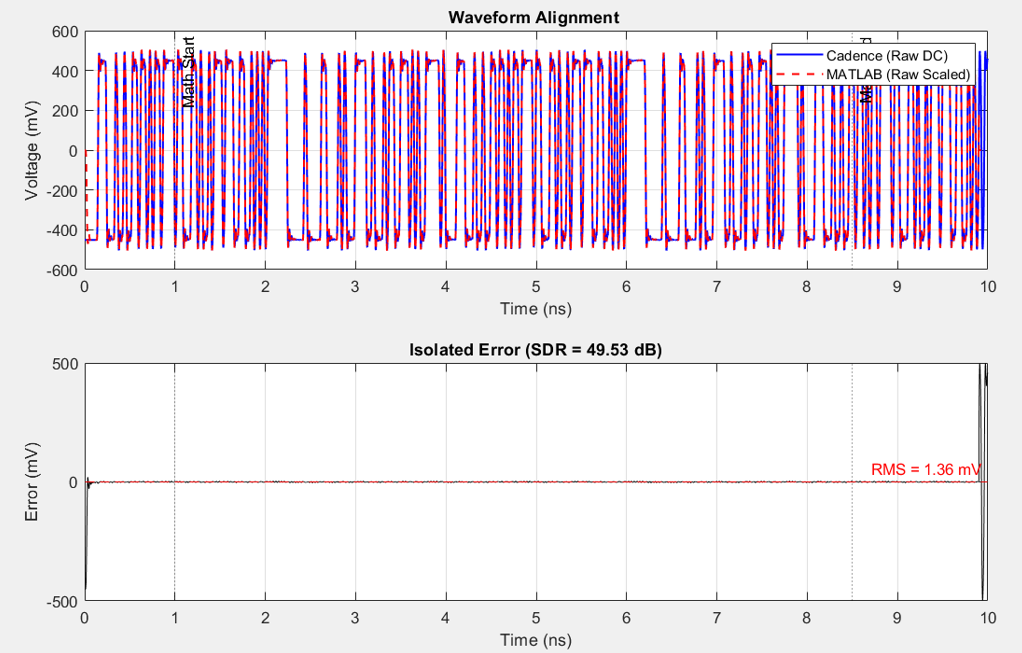
\includegraphics[width=0.8\textwidth]{img/TX_img/SDR_ideal.png}
    \caption{SDR measurement of the RC-equivalent model for linear reference validation.}
    \label{fig:sdr_ideal}
\end{figure}

The SDR measurement of the RC-model, presented in Figure~\ref{fig:sdr_ideal}, yields an SDR of $50~\text{dB}$, 
which serves as a baseline for the idealized linear behavior. This confirms that the residual error observed in the full driver-level simulation 
is indeed representative of the device non-linearities rather than inaccuracies in the behavioral model.



\subsection{AC Common-Mode Peak-to-Peak (AC CM PP) Analysis}

The transmitter common-mode voltage ($V_{CM} = (V_{D+} + V_{D-})/2$) is ideally constant in a balanced differential system. 
In practice, however, AC common-mode noise is generated primarily by physical imperfections during signal transitions:

\begin{enumerate}
    \item \textbf{Slew Rate Mismatch:} Asymmetry between the pull-up and pull-down network transition speeds causes 
    instantaneous current imbalances. As illustrated in Figure~\ref{fig:ac_cm_causes}, 
    this generates high-frequency ``shark-fin'' spikes in the common-mode voltage at every bit transition.
    \item \textbf{Amplitude Mismatch:} Discrepancies in the single-ended output swings lead to a lower-frequency, 
    persistent common-mode square wave. This offset effectively modulates the average common-mode level at the data rate, 
    resulting in a distinct ripple.
\end{enumerate}

\begin{figure}[H]
    \centering
    \begin{subfigure}[b]{0.48\textwidth}
        \centering
        
\includegraphics[width=\textwidth]{AC_CM_PP_Nominal.png}
        \caption{Nominal Corner}
    \end{subfigure}
    \hfill
    \begin{subfigure}[b]{0.48\textwidth}
        \centering
        
\includegraphics[width=\textwidth]{AC_CM_PP_SSmax.png}
        \caption{SSmax Corner}
    \end{subfigure}
    
    \vspace{0.3cm}
    
    \begin{subfigure}[b]{0.48\textwidth}
        \centering
        
\includegraphics[width=\textwidth]{AC_CM_PP_FS.png}
        \caption{FS Corner}
    \end{subfigure}
    \hfill
    \begin{subfigure}[b]{0.48\textwidth}
        \centering
        
\includegraphics[width=\textwidth]{AC_CM_PP_SF.png}
        \caption{SF Corner}
    \end{subfigure}
    \caption{AC common-mode voltage noise simulation results across process corners.}
    \label{fig:ac_cm_corners}
\end{figure}

The transmitter is verified against PCIe Gen 6.0 common-mode limits:
\begin{itemize}
    \item \textbf{Low-Frequency Limit:} Shall not exceed $25~\text{mV}_{\text{pp}}$ ($0.03\text{--}500~\text{MHz}$).
    \item \textbf{Nyquist Limit:} After applying a single-pole low-pass filter at the Nyquist frequency, shall not exceed $75~\text{mV}_{\text{pp}}$.
\end{itemize}

\begin{table}[H]
    \centering
    \caption{Simulated AC Common-Mode Peak-to-Peak Results}
    \label{tab:ac_cm_pp_results}
    \renewcommand{\arraystretch}{1.3}
    \begin{tabular}{lccc}
        \toprule
        \textbf{Corner} & \textbf{Bandpass ($0.03\text{--}500~\text{MHz}$)} & \textbf{Nyquist Filtered ($16~\text{GHz}$)} \\
        \midrule
        \textbf{Nominal} & $2.47~\text{mV}_{\text{pp}}$ & $15.74~\text{mV}_{\text{pp}}$ \\
        \textbf{SSmax}   & $2.22~\text{mV}_{\text{pp}}$ & $14.23~\text{mV}_{\text{pp}}$ \\
        \textbf{FS}      & $4.25~\text{mV}_{\text{pp}}$ & $26.73~\text{mV}_{\text{pp}}$ \\
        \textbf{SF}      & $0.71~\text{mV}_{\text{pp}}$ & $5.10~\text{mV}_{\text{pp}}$ \\
        \bottomrule
    \end{tabular}
\end{table}

The simulation results confirm that the transmitter maintains significant margin against the PCIe Gen 6.0 specification masks across all corners. 
The SF corner exhibits the most robust common-mode rejection, likely due to a self-compensating impedance balance between the PMOS and NMOS networks 
under asymmetric process skew.

\section{Layout Implementation}
\label{sec:layout}

This section details the physical implementation of the transmitter, focusing on the layout strategies employed to minimize parasitics 
and ensure signal integrity. The design follows a hierarchical approach, starting from fundamental gates and scaling up to the unit slice 
and final MSB driver array.

\subsection{Fundamental Gate Layouts}
The driver implementation relies on optimized layouts for the basic building blocks, ensuring symmetric matching and reduced interconnect parasitics. 

\begin{figure}[H]
    \centering
    \begin{subfigure}[b]{0.9\textwidth}
        \centering
        
\includegraphics[width=\textwidth]{Layout_Inverter.png}
        \caption{Inverter.}
    \end{subfigure}
    \hfill
    \begin{subfigure}[b]{0.9\textwidth}
        \centering
        
\includegraphics[width=\textwidth]{Layout_TG.png}
        \caption{Transmission Gate.}
    \end{subfigure}
    \hfill
    \begin{subfigure}[b]{0.9\textwidth}
        \centering
        
\includegraphics[width=\textwidth]{Layout_Series_N.png}
        \caption{Series N-MOS.}
    \end{subfigure}
    \hfill
    \begin{subfigure}[b]{0.9\textwidth}
        \centering
        
\includegraphics[width=\textwidth]{Layout_Series_P.png}
        \caption{Series P-MOS.}
    \end{subfigure}
    \caption{Fundamental gate layouts utilized in the transmitter driver.}
    \label{fig:fundamental_gates}
\end{figure}

\subsection{MSB Driver Layout First Iteration}
The MSB driver section utilizes a custom layout to manage the capacitive loading of the intermediate nodes. 
We first define the Single-Ended (SE) unit slice as the primary reference, followed by the complete MSB block.

\begin{figure}[H]
    \centering
    \begin{subfigure}[b]{0.9\textwidth}
        \centering
        
\includegraphics[width=\textwidth]{Layout_SE_Slice.png}
        \caption{Single-Ended (SE) unit slice layout.}
    \end{subfigure}
    \hfill
    \begin{subfigure}[b]{0.9\textwidth}
        \centering
        
\includegraphics[width=\textwidth]{Layout_MSB_first.png}
        \caption{MSB driver block layout.}
    \end{subfigure}
    \caption{MSB driver layout hierarchy.}
    \label{fig:msb_layout}
\end{figure}

\subsection{Parasitic Verification Results}
To validate the layout, we performed post-layout extraction (PEX) while selectively including parasitic RC components. 
Figure~\ref{fig:parasitic_results} illustrates the impact of excluding specific nodes (intermediate node, $V_{DD}$, $GND$, and $O/P$ pad) 
on the output voltage swing.

\begin{figure}[H]
    \centering
    \begin{subfigure}[b]{0.45\textwidth}
        \centering
        
\includegraphics[width=\textwidth]{Results_All_R.png}
        \caption{All parasitics included ($399~\text{mV}$).}
    \end{subfigure}
    \hfill
    \begin{subfigure}[b]{0.45\textwidth}
        \centering
        
\includegraphics[width=\textwidth]{Results_Exclude_Int.png}
        \caption{Exclude intermediate node ($421~\text{mV}$).}
    \end{subfigure}
    
    \vspace{0.5cm}
    
    \begin{subfigure}[b]{0.45\textwidth}
        \centering
        
\includegraphics[width=\textwidth]{Results_Exclude_Int_VDD_GND.png}
        \caption{Exclude intermediate node, $V_{DD}$, $GND$ ($434~\text{mV}$).}
    \end{subfigure}
    \hfill
    \begin{subfigure}[b]{0.45\textwidth}
        \centering
        
\includegraphics[width=\textwidth]{Results_Exclude_Int_VDD_GND_OP.png}
        \caption{Exclude intermediate node, $V_{DD}$, $GND$, $O/P$ ($449~\text{mV}$).}
    \end{subfigure}
    \caption{Post-layout simulation results showing the impact of parasitic node exclusion on output swing.}
    \label{fig:parasitic_results}
\end{figure}


\subsection{Layout Refinement and Parasitic Reduction}
\label{sec:layout_refinement}

To further optimize the driver performance, the layout was modified to minimize series resistance. 
This was achieved by increasing the via density and transitioning critical signal routing to higher metal layers with lower resistivity. 
The effectiveness of these modifications is verified by comparing the unit slice and MSB array layouts, followed by post-layout swing analysis.

\begin{figure}[H]
    \centering
    \begin{subfigure}[b]{0.9\textwidth}
        \centering
        
\includegraphics[width=\textwidth]{Layout_SE_Slice_modified.png}
        \caption{Modified Single-Ended (SE) unit slice.}
    \end{subfigure}
    \hfill
    \begin{subfigure}[b]{0.9\textwidth}
        \centering
        
\includegraphics[width=\textwidth]{Layout_MSB_modified.png}
        \caption{Modified MSB driver block layout.}
    \end{subfigure}
    \caption{Layout modifications for resistance reduction via via-stacking and higher metal routing.}
    \label{fig:modified_layout}
\end{figure}


Post-layout simulation of the modified driver indicates an improved output swing of $426~\text{mV}$, as shown in Figure~\ref{fig:swing_426}. 
The sensitivity analysis of parasitic node exclusion demonstrates significant improvements in performance after these layout optimizations:

\begin{figure}[H]
    \centering
    
\includegraphics[width=0.5\textwidth]{Results_swing_426mV.png}
    \caption{Improved output swing ($426~\text{mV}$) post-layout.}
    \label{fig:swing_426}
\end{figure}

\begin{itemize}
    \item \textbf{Intermediate Node:} Parasitic impact improved by $10.7~\text{mV}$ out of $22~\text{mV}$.
    \item \textbf{Output (O/P) Node:} Parasitic impact improved by $10~\text{mV}$ out of $15~\text{mV}$.
    \item \textbf{Supply and Ground ($V_{DD}$/GND):} Parasitic impact improved by $6~\text{mV}$ out of $12~\text{mV}$.
\end{itemize}


\newpage
\subsection{Full DAC Layout Integration and Verification}
\label{sec:full_layout}

The final physical integration of the design involves the assembly of the full DAC array, followed by the incorporation of the peaking inductors. 
Verification is performed using standard EDA tools to ensure physical and logical correctness.


    \begin{figure}[H]
        \centering
        
\includegraphics[width=0.9\textwidth]{Full_DAC_Layout.png}
        \caption{Complete DAC layout array.}
    \end{figure}

    \begin{figure}[H]
        \centering
        
\includegraphics[width=0.9\textwidth]{Full_DAC_wz_inductor_Layout.png}
        \caption{DAC with integrated peaking inductors.}
    \end{figure}

    \begin{figure}[H]
        \centering
        
\includegraphics[width=0.9\textwidth]{LAYOUT_AREA.png}
        \caption{Layout_Area.}
    \end{figure}

    \begin{itemize}
    \item Area without inductor = $70~\mu\text{m} \times 60~\mu\text{m} = 4200~\mu\text{m}^2$
    \item Area with inductor = $240~\mu\text{m} \times 122.5~\mu\text{m} = 29,400~\mu\text{m}^2$
    \end{itemize}
  
\subsection{Parasitic Scaling and Fractional Dummy Insertion}
To maintain strict binary weighting across the DAC branches, the routing parasitics must scale proportionally with the transistor widths. 
For the Most Significant Bits (MSBs, e.g., B7 and B6), the full active width (32 units) is utilized for both the Inverter and the Transmission Gate (TG). 
However, for the lower bits (e.g., B5), the required active width is halved (16 units). 

Simply shrinking the layout footprint would disrupt the pitch and create severe Layout Dependent Effect (LDE) mismatches. Instead, 
the lower bits maintain the identical physical footprint of the MSBs, but half of the transistor fingers are deactivated to serve as dummy devices. 

The placement of these active fingers is critical to ensure the input ($i/p$) and output ($o/p$) routing parasitics scale linearly. 
Three primary placement topologies were considered, as illustrated in Figure~\ref{fig:dummy_insertion}:

\begin{enumerate}
    \item \textbf{Case 1 (Left-Aligned):} The first half of both devices is active. While this minimizes the input routing length, 
    the output signal must traverse the entire dummy section of the TG to reach the common output bus, destroying the parasitic scaling ratio.
    \item \textbf{Case 2 (Right-Aligned):} The second half is active. This minimizes the output routing, 
    but forces the input signal to route over the dummy inverter fingers, creating an analogous parasitic imbalance at the input node.
    \item \textbf{Case 3 (Edge-Aligned / Optimal):} The active fingers are pushed to the extreme outer edges—the first half of the Inverter 
    and the second half of the TG are active. This perfectly scales both the input and output routing lengths by a factor of two, perfectly 
    matching the 16-unit electrical width while isolating the active devices from internal cross-coupling.
\end{enumerate}

\begin{figure}[H]
    \centering
    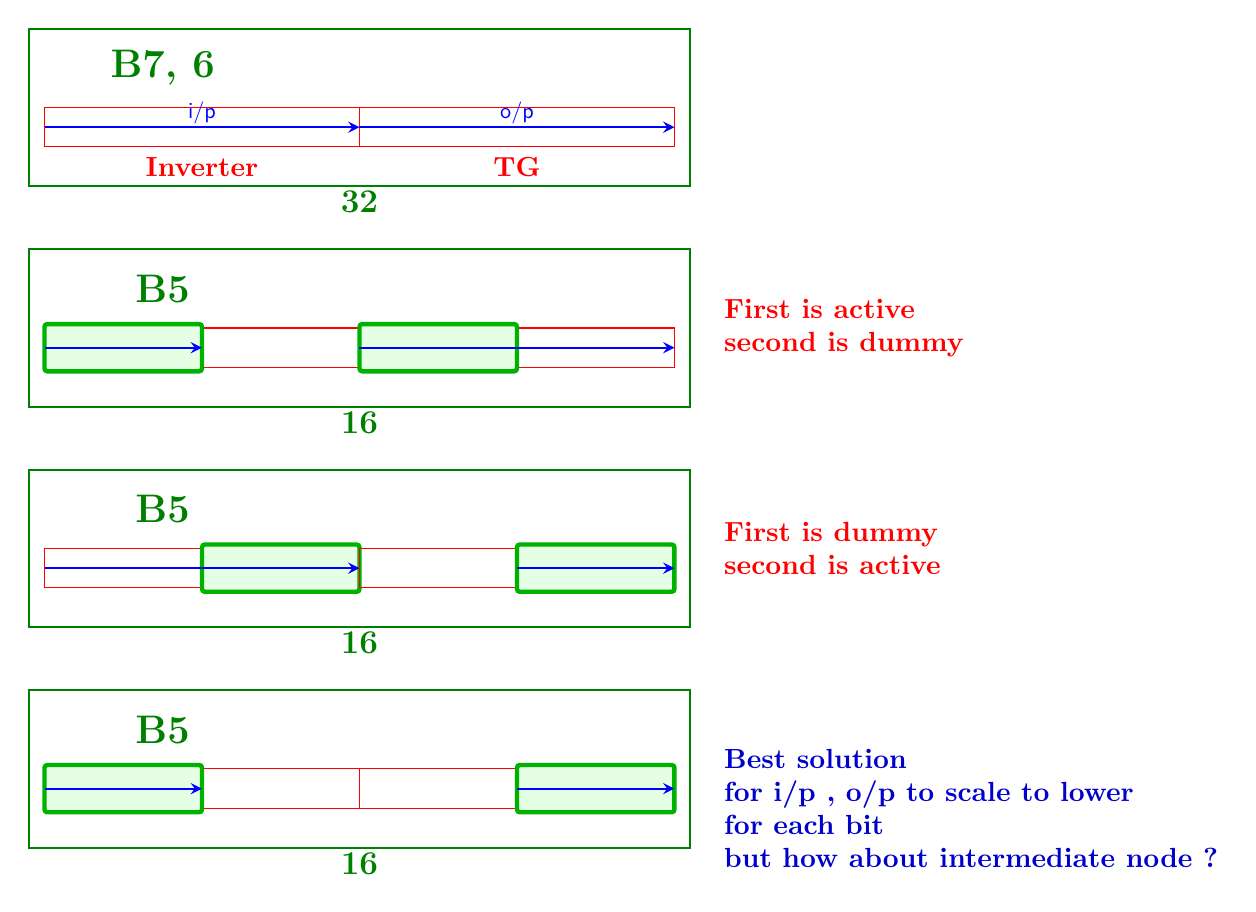
\begin{tikzpicture}[
        thick,
        activebox/.style={draw=green!70!black, ultra thick, fill=green!10, rounded corners=1pt},
        dummybox/.style={draw=red, thin},
        arrow/.style={blue, ->, >=stealth, thick},
        font=\sffamily
    ]

    % ==========================================
    % ROW 1: B7, 6 (MSB - Full Width 32)
    % ==========================================
    \begin{scope}[yshift=0cm]
        \draw[thick, green!50!black] (-0.2, -0.5) rectangle (8.2, 1.5);
        \node[text=green!50!black, font=\Large\bfseries] at (1.5, 1) {B7, 6};
        
        \draw[dummybox] (0,0) rectangle (4,0.5); % Inverter
        \draw[dummybox] (4,0) rectangle (8,0.5); % TG
        
        \draw[arrow] (0,0.25) -- (4,0.25) node[midway, above=-2pt, scale=0.8] {i/p};
        \draw[arrow] (4,0.25) -- (8,0.25) node[midway, above=-2pt, scale=0.8] {o/p};
        
        \node[text=red, font=\bfseries] at (2, -0.25) {Inverter};
        \node[text=red, font=\bfseries] at (6, -0.25) {TG};
        \node[text=green!50!black, font=\large\bfseries] at (4, -0.7) {32};
    \end{scope}

    % ==========================================
    % ROW 2: B5 (Case 1: First is active)
    % ==========================================
    \begin{scope}[yshift=-2.8cm]
        \draw[thick, green!50!black] (-0.2, -0.5) rectangle (8.2, 1.5);
        \node[text=green!50!black, font=\Large\bfseries] at (1.5, 1) {B5};
        
        % Inverter
        \draw[dummybox] (0,0) rectangle (4,0.5); 
        \filldraw[activebox] (0,-0.05) rectangle (2,0.55);
        \draw[arrow] (0,0.25) -- (2,0.25);
        
        % TG
        \draw[dummybox] (4,0) rectangle (8,0.5);
        \filldraw[activebox] (4,-0.05) rectangle (6,0.55);
        \draw[arrow] (4,0.25) -- (8,0.25); % Routes through dummy
        
        \node[text=green!50!black, font=\large\bfseries] at (4, -0.7) {16};
        \node[text=red, font=\bfseries, align=left, right] at (8.5, 0.5) {First is active\\second is dummy};
    \end{scope}

    % ==========================================
    % ROW 3: B5 (Case 2: Second is active)
    % ==========================================
    \begin{scope}[yshift=-5.6cm]
        \draw[thick, green!50!black] (-0.2, -0.5) rectangle (8.2, 1.5);
        \node[text=green!50!black, font=\Large\bfseries] at (1.5, 1) {B5};
        
        % Inverter
        \draw[dummybox] (0,0) rectangle (4,0.5);
        \filldraw[activebox] (2,-0.05) rectangle (4,0.55);
        \draw[arrow] (0,0.25) -- (4,0.25); % Routes through dummy
        
        % TG
        \draw[dummybox] (4,0) rectangle (8,0.5);
        \filldraw[activebox] (6,-0.05) rectangle (8,0.55);
        \draw[arrow] (6,0.25) -- (8,0.25);
        
        \node[text=green!50!black, font=\large\bfseries] at (4, -0.7) {16};
        \node[text=red, font=\bfseries, align=left, right] at (8.5, 0.5) {First is dummy\\second is active};
    \end{scope}

    % ==========================================
    % ROW 4: B5 (Case 3: Edge-Aligned / Best)
    % ==========================================
    \begin{scope}[yshift=-8.4cm]
        \draw[thick, green!50!black] (-0.2, -0.5) rectangle (8.2, 1.5);
        \node[text=green!50!black, font=\Large\bfseries] at (1.5, 1) {B5};
        
        % Inverter
        \draw[dummybox] (0,0) rectangle (4,0.5);
        \filldraw[activebox] (0,-0.05) rectangle (2,0.55);
        \draw[arrow] (0,0.25) -- (2,0.25);
        
        % TG
        \draw[dummybox] (4,0) rectangle (8,0.5);
        \filldraw[activebox] (6,-0.05) rectangle (8,0.55);
        \draw[arrow] (6,0.25) -- (8,0.25);
        
        \node[text=green!50!black, font=\large\bfseries] at (4, -0.7) {16};
        \node[text=blue!80!black, font=\bfseries, align=left, right] at (8.5, 0) {Best solution\\for i/p , o/p to scale to lower\\for each bit\\but how about intermediate node ?};
    \end{scope}

    \end{tikzpicture}
    \caption{Fractional dummy insertion strategies for lower DAC bits to maintain parasitic scaling.}
    \label{fig:dummy_insertion}
\end{figure}

While the edge-aligned topology (Case 3) perfectly optimizes the parasitic scaling for the external input and output nodes, it introduces a severe penalty for the internal connection. By pushing the active Inverter fingers to the far left and the active TG fingers to the far right, the physical routing distance \textit{between} the two stages is effectively doubled. 

To minimize the intermediate node capacitance, the active devices must be placed as close together as possible. As shown in Figure~\ref{fig:intermediate_node}, the optimal solution for the intermediate node is to activate the second half of the Inverter and the first half of the TG. 

\begin{figure}[H]
    \centering
    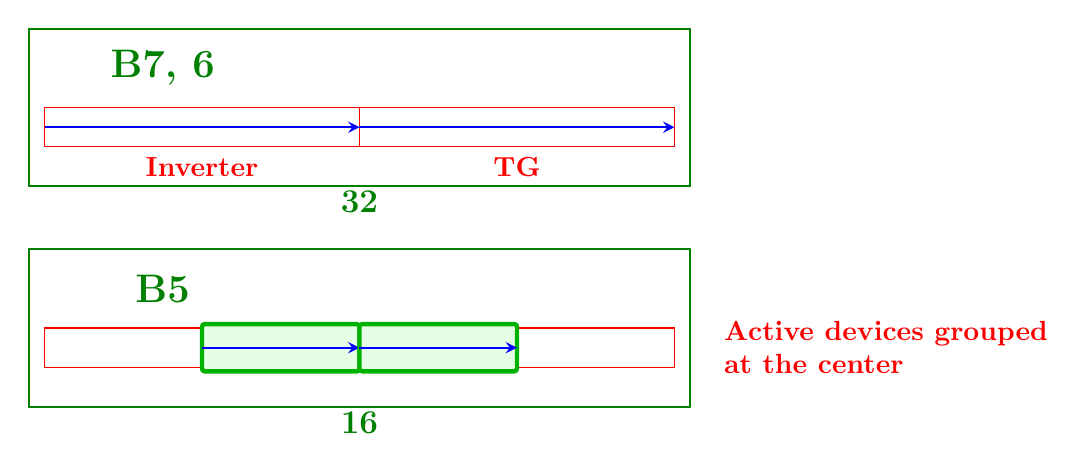
\begin{tikzpicture}[
        thick,
        activebox/.style={draw=green!70!black, ultra thick, fill=green!10, rounded corners=1pt},
        dummybox/.style={draw=red, thin},
        arrow/.style={blue, ->, >=stealth, thick},
        font=\sffamily
    ]

    % ==========================================
    % ROW 1: B7, 6 (MSB - Full Width 32)
    % ==========================================
    \begin{scope}[yshift=0cm]
        \draw[thick, green!50!black] (-0.2, -0.5) rectangle (8.2, 1.5);
        \node[text=green!50!black, font=\Large\bfseries] at (1.5, 1) {B7, 6};
        
        \draw[dummybox] (0,0) rectangle (4,0.5); % Inverter
        \draw[dummybox] (4,0) rectangle (8,0.5); % TG
        
        \draw[arrow] (0,0.25) -- (4,0.25);
        \draw[arrow] (4,0.25) -- (8,0.25);
        
        \node[text=red, font=\bfseries] at (2, -0.25) {Inverter};
        \node[text=red, font=\bfseries] at (6, -0.25) {TG};
        \node[text=green!50!black, font=\large\bfseries] at (4, -0.7) {32};
    \end{scope}

    % ==========================================
    % ROW 2: B5 (Centered Active - Best for Intermediate Node)
    % ==========================================
    \begin{scope}[yshift=-2.8cm]
        \draw[thick, green!50!black] (-0.2, -0.5) rectangle (8.2, 1.5);
        \node[text=green!50!black, font=\Large\bfseries] at (1.5, 1) {B5};
        
        % Inverter
        \draw[dummybox] (0,0) rectangle (4,0.5); 
        \filldraw[activebox] (2,-0.05) rectangle (4,0.55);
        \draw[arrow] (2,0.25) -- (4,0.25);
        
        % TG
        \draw[dummybox] (4,0) rectangle (8,0.5);
        \filldraw[activebox] (4,-0.05) rectangle (6,0.55);
        \draw[arrow] (4,0.25) -- (6,0.25); 
        
        \node[text=green!50!black, font=\large\bfseries] at (4, -0.7) {16};
        \node[text=red, font=\bfseries, align=left, right] at (8.5, 0.25) {Active devices grouped\\at the center};
    \end{scope}

    \end{tikzpicture}
    \caption{Optimal active finger placement to minimize the intermediate node routing capacitance.}
    \label{fig:intermediate_node}
\end{figure}

This arrangement groups all active layout regions at the center of the footprint, minimizing the internal routing wire length. However, this creates a direct architectural conflict: the layout strategy that represents the best-case scenario for the intermediate node is the exact worst-case scenario for the external input and output scaling. The input signal must now route over the dummy Inverter fingers to reach the active devices, and the output signal must similarly traverse the dummy TG fingers to reach the common rail. This conflict dictates that the final layout cannot perfectly optimize both domains simultaneously, necessitating a careful design trade-off based on which parasitic capacitance (internal vs. external) dominates the overall driver bandwidth and return loss.
\subsection*{Final Layout Strategy: Node Prioritization}
Because it is physically impossible to simultaneously optimize the input, intermediate, and output nodes, a strategic trade-off is required. The decision must be driven by the electrical sensitivity of each node to parasitic capacitance. The following prioritization scheme was established for the fractional dummy insertion:

\begin{enumerate}
    \item \textbf{Input Node (Highest Priority):} Must perfectly scale to maintain the precise binary weighting of the input capacitance presented to the preceding pre-driver stage.
    \item \textbf{Intermediate Node (High Priority):} The internal connection between the Inverter and the Transmission Gate (TG) is highly sensitive. Excess parasitic capacitance here acts as a dominant pole, severely degrading the internal slew rate and bandwidth of the driver branch.
    \item \textbf{Output Node (Lowest Priority):} The routing capacitance at the final output node is less critical because it is positioned before the series termination resistor ($R$). The resistor effectively masks a portion of this capacitance from the main transmission line, mitigating its impact on the overall return loss compared to the internal nodes.
\end{enumerate}

Based on this prioritization, the final chosen topology activates the \textit{first half} of both the Inverter and the TG (Case 1 from the initial analysis). As illustrated in Figure~\ref{fig:final_node_priority}, this achieves the perfect $0.5\times$ scaling for the critical input node. The intermediate node routing distance scales by $0.75\times$, offering a strong compromise that preserves internal bandwidth. The output node takes the penalty with a $1.0\times$ scaling (no reduction), which is an acceptable trade-off given its lower electrical priority.

Because it is physically impossible to simultaneously optimize the input, intermediate, and output nodes, a strategic trade-off is required. The decision must be driven by the electrical sensitivity of each node to parasitic capacitance. The following prioritization scheme was established for the fractional dummy insertion:

\begin{enumerate}
    \item \textbf{Input Node (Highest Priority):} Must perfectly scale to maintain the precise binary weighting of the input capacitance presented to the preceding pre-driver stage.
    \item \textbf{Intermediate Node (High Priority):} The internal connection between the Inverter and the Transmission Gate (TG) is highly sensitive. Excess parasitic capacitance here acts as a dominant pole, severely degrading the internal slew rate and bandwidth of the driver branch.
    \item \textbf{Output Node (Lower Priority):} The routing capacitance at the final output node is less critical because it is positioned before the series termination resistor ($R$). The resistor effectively masks a portion of this capacitance from the main transmission line, mitigating its impact on the overall return loss compared to the internal nodes.
\end{enumerate}

The final chosen topology activates the \textit{first half} of both the Inverter and the TG. As illustrated in Figure~\ref{fig:final_node_priority}, this arrangement yields the following scaling factors for the layout parasitics relative to the MSB:
\begin{itemize}
    \item \textbf{Input (i/p) node:} $0.5\times$
    \item \textbf{Intermediate node:} $0.75\times$
    \item \textbf{Output (o/p) node:} $1.0\times$
\end{itemize}

By prioritizing the input node, perfect scaling is achieved for the most sensitive capacitance. The intermediate node takes the next priority with a $0.75\times$ scaling factor, offering a strong compromise to preserve internal bandwidth. The output node takes the penalty with a $1.0\times$ scaling (no reduction). Because the output capacitance under consideration lies strictly \textit{before} the series termination resistor, this prioritization is the optimal choice; the resistor effectively shields the external transmission line from this unscaled capacitance.

\begin{figure}[H]
    \centering
    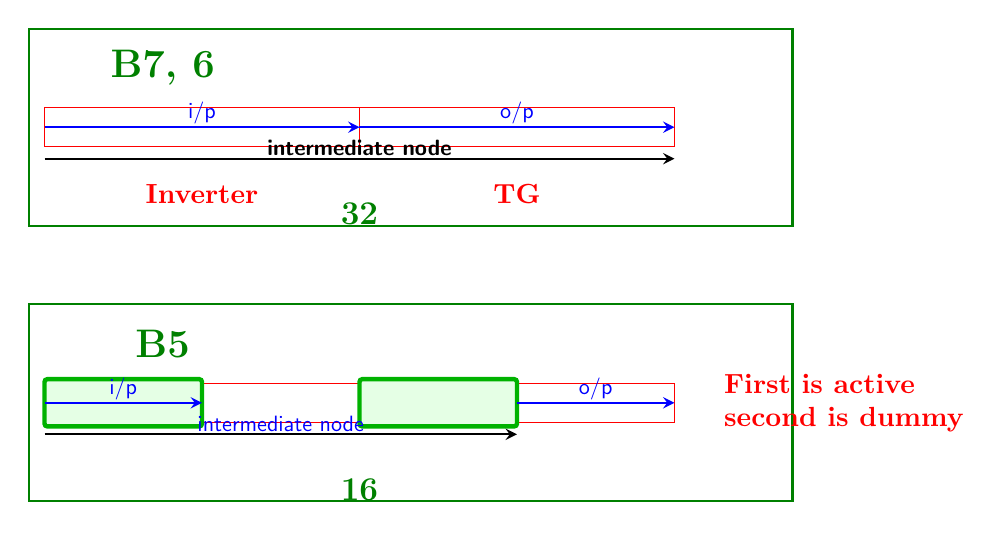
\begin{tikzpicture}[
        thick,
        activebox/.style={draw=green!70!black, ultra thick, fill=green!10, rounded corners=1pt},
        dummybox/.style={draw=red, thin},
        arrow/.style={blue, ->, >=stealth, thick},
        blackarrow/.style={black, ->, >=stealth, thick},
        font=\sffamily
    ]

    % ==========================================
    % ROW 1: B7, 6 (MSB - Full Width 32)
    % ==========================================
    \begin{scope}[yshift=0cm]
        \draw[thick, green!50!black] (-0.2, -1.0) rectangle (9.5, 1.5);
        \node[text=green!50!black, font=\Large\bfseries] at (1.5, 1) {B7, 6};
        
        \draw[dummybox] (0,0) rectangle (4,0.5); % Inverter
        \draw[dummybox] (4,0) rectangle (8,0.5); % TG
        
        \draw[arrow] (0,0.25) -- (4,0.25) node[midway, above=-2pt, scale=0.8] {i/p};
        \draw[arrow] (4,0.25) -- (8,0.25) node[midway, above=-2pt, scale=0.8] {o/p};
        \draw[blackarrow] (0,-0.15) -- (8,-0.15) node[midway, above=-2pt, scale=0.8] {\textbf{intermediate node}};
        
        \node[text=red, font=\bfseries] at (2, -0.6) {Inverter};
        \node[text=red, font=\bfseries] at (6, -0.6) {TG};
        \node[text=green!50!black, font=\large\bfseries] at (4, -0.85) {32};
    \end{scope}

    % ==========================================
    % ROW 2: B5 (Final Choice)
    % ==========================================
    \begin{scope}[yshift=-3.5cm]
        \draw[thick, green!50!black] (-0.2, -1.0) rectangle (9.5, 1.5);
        \node[text=green!50!black, font=\Large\bfseries] at (1.5, 1) {B5};
        
        % Inverter
        \draw[dummybox] (0,0) rectangle (4,0.5); 
        \filldraw[activebox] (0,-0.05) rectangle (2,0.55);
        \draw[arrow] (0,0.25) -- (2,0.25) node[midway, above=-2pt, scale=0.8] {i/p};
        
        % TG
        \draw[dummybox] (4,0) rectangle (8,0.5);
        \filldraw[activebox] (4,-0.05) rectangle (6,0.55);
        \draw[arrow] (6,0.25) -- (8,0.25) node[midway, above=-2pt, scale=0.8] {o/p}; 
        
        % Intermediate node arrow: starts from 0, ends at 6 (75% of total width)
        \draw[blackarrow] (0,-0.15) -- (6,-0.15) node[midway, above=-2pt, scale=0.8, text=blue] {intermediate node};
        
        \node[text=green!50!black, font=\large\bfseries] at (4, -0.85) {16};
        \node[text=red, font=\bfseries, align=left, right] at (8.5, 0.25) {First is active\\second is dummy};
    \end{scope}

    \end{tikzpicture}
    \caption{Final fractional dummy insertion strategy demonstrating the routing lengths for the prioritized nodes.}
    \label{fig:final_node_priority}
\end{figure}


\subsubsection{Layout Verification}
To ensure the integrity of the design, rigorous design rule checking (DRC) and layout-versus-schematic (LVS) verification were 
performed using Siemens EDA tools. The results in Figure~\ref{fig:verification_results} confirm a clean, error-free layout ready for fabrication.

% --- DRC Results ---
\begin{figure}[H]
    \centering
    \begin{subfigure}[b]{0.45\textwidth}
        \centering
        
\includegraphics[width=\textwidth]{DRC1.png}
        \caption{Design Rule Check (DRC) Part 1.}
    \end{subfigure}
    \hfill
    \begin{subfigure}[b]{0.45\textwidth}
        \centering
        
\includegraphics[width=\textwidth]{DRC2.png}
        \caption{Design Rule Check (DRC) Part 2.}
    \end{subfigure}
    \caption{Design Rule Check (DRC) verification results.}
    \label{fig:drc_results}
\end{figure}

% --- LVS Results ---
\begin{figure}[H]
    \centering
    
\includegraphics[width=0.6\textwidth]{LVS.png}
    \caption{Layout-Versus-Schematic (LVS) verification results.}
    \label{fig:lvs_results}
\end{figure}


The verification reports confirm that all design rules, including antenna and density requirements, have been met. 
The LVS check matches the extracted layout to the design schematic, ensuring logical equivalence for high-speed operation.

\section{Post Layout Simultion}
\subsection{Post-Layout Swing Specification Verification}
\label{sec:post_layout_swing}

Following the physical implementation and parasitic extraction, the output voltage swing was re-verified to ensure that 
the design maintains compliance with the specified $0.8~\text{V}$ to $1.0~\text{V}$ (differential) range. 
This post-layout simulation accounts for the parasitic resistance and capacitance introduced by the routing and via stacks.

\begin{figure}[H]
    \centering
    
\includegraphics[width=0.9\textwidth]{Swing_Post_Layout.png}
    \caption{Post-layout simulation of the differential output voltage swing across process corners.}
    \label{fig:swing_post_layout}
\end{figure}

The post-layout results demonstrate that the driver maintains a consistent differential swing across all process corners. 
The analysis confirms that the impact of layout parasitics has been successfully minimized, preserving the signal integrity and 
voltage levels established in the pre-layout design phase. The design remains robust against PVT variations, 
meeting all target output swing specifications required for reliable operation.
\subsection{Post-Layout PAM-4 Eye Diagram Analysis}
\label{sec:pam4_post_layout}

The PAM-4 eye diagrams were simulated post-layout to verify signal integrity under realistic parasitic conditions. The linearity, 
quantified by the Ratio Level Mismatch (RLM), demonstrates that the design maintains excellent eye symmetry.

\begin{figure}[H]
    \centering
    \begin{subfigure}[b]{0.48\textwidth}
        \centering
        
\includegraphics[width=\textwidth]{Nominal_EYE_Post_Layout.png}
        \caption{Nominal corner (RLM $\approx 96.8\%$).}
    \end{subfigure}
    \hfill
    \begin{subfigure}[b]{0.48\textwidth}
        \centering
        
\includegraphics[width=\textwidth]{SSmax_EYE_Post_Layout.png}
        \caption{SS Max corner (RLM $\approx 95.5\%$).}
    \end{subfigure}
    \caption{Post-layout PAM-4 eye diagrams and linearity verification.}
    \label{fig:pam4_post_layout}
\end{figure}

The RLM values of $96.8\%$ and $95.5\%$ for the nominal and SS-Max corners, respectively, confirm that the modulated design successfully 
minimizes level mismatch, ensuring high-quality multilevel signaling even under process variations.

\subsection{Post-Layout Return Loss Analysis}
\label{sec:post_layout_rl}

The physical layout parasitics, including interconnect routing and via resistances, significantly impact the impedance matching of the transmitter. 
To verify the performance of the modulated design post-layout, both differential return loss ($S_{dd11}$) and common-mode return loss ($S_{11CM}$) 
were simulated across various process corners (Nominal, SS-Max, and FF-Min).

\begin{figure}[H]
    \centering
    
\includegraphics[width=0.8\textwidth]{Sd11_post_layout.png}
    \caption{Post-layout differential return loss ($S_{dd11}$) across process corners.}
    \label{fig:post_layout_sdd11}
\end{figure}

\begin{figure}[H]
    \centering
    
\includegraphics[width=0.8\textwidth]{S11CM_post_layout.png}
    \caption{Post-layout common-mode return loss ($S_{11CM}$) across process corners.}
    \label{fig:post_layout_s11cm}
\end{figure}

\begin{figure}[H]
    \centering
    
\includegraphics[width=0.8\textwidth]{Rdiff_Post_Layout.png}
    \caption{O/P impedance}
   
\end{figure}

The post-layout results demonstrate that the transmitter maintains robust impedance matching across the operating bandwidth. 
The differential return loss remains well-contained, and the common-mode suppression validates the effectiveness of the layout strategy 
in maintaining signal integrity and minimizing undesired reflections despite the introduced parasitic elements.


\newpage
\section{Improved Design}
\label{sec:modulated_design}

To enhance the performance of the calibration DAC, an additional branch was introduced to decrease the calibration step size. 
This approach provides finer control over the output impedance tuning. As shown in Figure~\ref{fig:mod_schematic}, 
the design utilizes a high-resistance $R_{branch}$ configuration. By implementing a significantly higher resistance compared to the baseline, 
the contribution of the MOSFETs to the overall path is minimized, effectively negating the need for additional transistor-based switching 
in this specific branch.

\begin{figure}[H]
    \centering
    
\includegraphics[width=1.1\textwidth]{Modulated_design_schematic.png}
    \caption{Schematic of the modulated DAC design with an additional calibration branch.}
    \label{fig:mod_schematic}
\end{figure}

The calibration strategy was verified through parameter interpolation across various process corners, as illustrated in Figure~\ref{fig:cal_curve}. 
The design demonstrates consistent behavior throughout the interpolation steps.

\begin{figure}[H]
    \centering
    
\includegraphics[width=0.9\textwidth]{Callibration graph.png}
    \caption{Parameter interpolation across process corners.}
    \label{fig:cal_curve}
\end{figure}

The mathematical validation of the interpolation steps is confirmed by the following equations, demonstrating the target resistance of $320~\Omega$:

\begin{equation}
    (1): \frac{395 \times R_{bank} \times \frac{395}{470}}{395 + R_{bank} \times \frac{395}{470}} = 320~\Omega
\end{equation}
\begin{flushleft}
    Where $R_{bank} \approx 2005~\Omega$, and $R_{branch} = 470 \times 4 \cdot R_{poly} + 125 \text{ (TG)}$.
\end{flushleft}

\begin{equation}
    (2): \frac{545 \times (2005 \parallel 1003) \times \frac{545}{470}}{545 + (2005 \parallel 1003) \times \frac{545}{470}} = 320~\Omega
\end{equation}
\subsection{Swing Performance and Supply Variation Analysis}


To ensure the effectiveness of the added calibration branch, the transmitter was evaluated under varying supply voltage conditions. 
The primary design objective was to match the sizing of $R_{main}$ ($395~\Omega$) to the rest of the resistor bank, 
ensuring that the variations across the Typical-Typical (TT) process corner—spanning min, nom, and max conditions—remain consistent.
Notice that typical/Nominal here means this process corner (1) not TT
\begin{figure}[H]
    \centering
    \begin{subfigure}[b]{0.5\textwidth}
        \centering
        
\includegraphics[width=\textwidth]{Swing_Fig1.png}
        \caption{Swing at $10\%$ supply variation.}
    \end{subfigure}
    \hfill
    \begin{subfigure}[b]{0.45\textwidth}
        \centering
        
\includegraphics[width=\textwidth]{Swing_Fig2.png}
        \caption{Swing with $R_{main} = 432.5~\Omega$ and scaled $R_{bank}$.}
    \end{subfigure}
    \caption{Output swing performance analysis under supply voltage variations.}
    \label{fig:mod_swing_results}
\end{figure}

The simulation results in Figure~\ref{fig:mod_swing_results} demonstrate the calibration range capability:

\begin{itemize}
    \item \textbf{Figure~\ref{fig:mod_swing_results}(a):} Represents the swing performance under a $10\%$ supply voltage variation with $R_{main}$ 
    set to $395~\Omega$.
    \item \textbf{Figure~\ref{fig:mod_swing_results}(b):} To evaluate the coverage of the calibration code, $R_{main}$ was set to 
    $432.5~\Omega$ (the midpoint between $395~\Omega$ and $420~\Omega$) and the calibration bank resistance ($R_{bank}$) was scaled by the variation ratio. The results confirm that the design successfully covers the target range up to a supply variation of approximately $8.5\%$.
\end{itemize}

This verification confirms that the modulated design maintains sufficient tuning range to compensate for supply-induced fluctuations, 
validating the sizing strategy employed for the additional calibration branch.


\subsection{PAM-4 Signaling and Linearity Analysis}
\label{sec:pam4_analysis}

The PAM-4 signaling scheme provides double the data rate of NRZ by utilizing four distinct voltage levels. 
To ensure signal integrity, the Ratio Level Mismatch (RLM) is characterized across nominal, maximum, and minimum process conditions. 
The resulting eye diagrams and corresponding RLM values are presented in Figure~\ref{fig:pam4_eyes}.

\begin{figure}[H]
    \centering
    \begin{subfigure}[b]{0.45\textwidth}
        \centering
        
\includegraphics[width=\textwidth]{PAM4_Nominal.png}
        \caption{this process corner corner (RLM = $98.3\%$).}
    \end{subfigure}
    \hfill
    \begin{subfigure}[b]{0.45\textwidth}
        \centering
        
\includegraphics[width=\textwidth]{PAM4_Max.png}
        \caption{Maximum corner (RLM = $98.87\%$).}
    \end{subfigure}
    
    \vspace{0.5cm}
    
    \begin{subfigure}[b]{0.45\textwidth}
        \centering
        
\includegraphics[width=\textwidth]{PAM4_Min.png}
        \caption{Minimum corner (RLM = $98.4\%$).}
    \end{subfigure}
    \caption{PAM-4 eye diagram analysis and RLM verification across process corners.}
    \label{fig:pam4_eyes}
\end{figure}

The high RLM values observed (greater than $98\%$) confirm excellent linearity and uniform eye opening across all process corners, 
validating the transmitter's capability to maintain high signal quality in PAM-4 operation.
\subsection{Return Loss and Differential Impedance Analysis}
\label{sec:freq_analysis}

To ensure optimal signal transmission and minimal reflections, the transmitter's return loss and differential impedance were characterized 
across the frequency spectrum. Figure~\ref{fig:return_loss_impedance} shows the simulation results for both the differential return loss ($S_{dd11}$) 
and the differential impedance ($R_{diff}$) for this process corner.

\begin{figure}[H]
    \centering
    \begin{subfigure}[b]{0.48\textwidth}
        \centering
        
\includegraphics[width=\textwidth]{Return_Loss_modulated_Plot.png}
        \caption{Differential return loss ($S_{dd11}$) vs. frequency.}
    \end{subfigure}
    \hfill
    \begin{subfigure}[b]{0.48\textwidth}
        \centering
        
\includegraphics[width=\textwidth]{Rdiff_modulated_Plot.png}
        \caption{Differential impedance ($R_{diff}$) vs. frequency.}
    \end{subfigure}
    \caption{Frequency-domain analysis of transmitter return loss and differential impedance.}
    \label{fig:return_loss_impedance}
\end{figure}

The differential return loss indicates high signal fidelity with substantial suppression of reflections across the target frequency range. 
Concurrently, the differential impedance profile demonstrates a stable matching characteristic, 
maintaining robustness against process variations within the operational bandwidth.

